\pagebreak
\section{The Extraction Decision: When to Migrate?}
\label{sec:extraction-decision}

The six guidelines G1 to G6 prepare a modular monolith for extraction. The preparation comes in two forms. G3 (Design for Progressive Scalability) provides \emph{structural readiness} through the Progressive Scalability Spectrum and the composite extraction readiness gate $\varepsilon_m$, which together signal whether a module's contracts and dependencies are mature enough to be separated from the monolith. G4 (Promote Migration Readiness) provides \emph{operational readiness} through Anti-Corruption Layers, sagas, and durable event delivery, which ensure that the extraction does not require a code rewrite at the moment it is triggered. Together, structural and operational readiness answer the question: \emph{is this module ready to be extracted?} They do not, by themselves, answer the prior question: \emph{should this module be extracted now?} Readiness without a justifying outcome leads to premature distribution; pursuing extraction without operational readiness leads to a distributed monolith. This section synthesizes the two questions into a single decision framework that draws on Khononov's Balanced Coupling model~\cite{khononov2024balancing} and Newman's extraction guidance~\cite{newman2019monolith}.

\subsection*{The Six-Question Checklist}

The decision to extract a module is justified when all six of the following questions can be answered in the affirmative. Questions one and two are structural signals derived from Khononov's coupling model. Questions three to five are strategic signals derived from Newman's Three Key Questions. Question six is an organizational signal derived from Newman's saga-style guidance.

\begin{enumerate}[itemsep=8pt,topsep=2pt]
  \item \emph{Is the Integration Strength low and stable?} The Integration Strength Index (ISI), defined in G2 (Embed Maintainability) as the ratio of contract-level integration points to the total cross-module integration points, must be at or above the target of $0.8$. When the ISI is high, most cross-module interactions are mediated by explicit contracts, and the candidate module exposes little intrusive or functional coupling that would survive the extraction as distributed-monolith debt.

  \item \emph{Is the Strength-Distance gap balanced by Volatility?} Khononov's coupling model relates three properties of any two interacting modules: integration \emph{Strength} (how tightly the modules are coupled), \emph{Distance} (how separated they are organizationally and procedurally), and \emph{Volatility} (how often their contracts change)~\cite{khononov2024balancing}. A module that is structurally distant from its peers (different team, different release cadence) but volatile in its contracts is a poor extraction candidate: every contract change becomes coordination cost across the network boundary. Extraction is justified when low strength and low volatility allow the distance between modules to grow without triggering coordination overhead.

  \item \emph{What outcome does extraction enable that the modular monolith cannot deliver?} This is the first of Newman's Three Key Questions~\cite{newman2019monolith}. Concrete answers include independent scaling beyond what the G3 L2 Isolate tier (a dedicated database schema per module within the same deployment) supports, an independent release cadence that removes a deployment bottleneck, or fault isolation that an in-process module cannot provide. Vague answers such as ``microservices are modern'' or ``the team wants experience with distributed systems'' fail this question.

  \item \emph{Have alternatives to extraction been considered and ruled out?} This is the second of Newman's Three Key Questions. Alternatives include vertical scaling, caching, read replicas, and the intermediate tiers of the G3 Scalability Spectrum: L1 Decouple (asynchronous boundaries that absorb load spikes within the monolith) and L2 Isolate (a dedicated database schema per module while keeping a single deployment target). Extraction is the most expensive option in the spectrum and should be selected only when these cheaper options cannot meet the outcome identified in question three.

  \item \emph{Does the team have the capability to operate a distributed system?} This is the third of Newman's Three Key Questions. Capability requires distributed tracing through correlation identifiers (introduced in G6, Introduce Observability Patterns), durable event delivery with versioned contracts (introduced in G4, Promote Migration Readiness), prior saga implementation experience, and an on-call rotation prepared for cross-service incident response. A team that cannot debug a distributed failure in production should not extract a module.

  \item \emph{Which saga coordination style fits the team topology?} Section~\ref{sec:g4-saga-styles} introduced the choice between an orchestrated saga, where a central component drives every step in sequence, and a choreographed saga, where each module reacts to events on a shared bus. A single team owning the full workflow can adopt the orchestrated style without crossing team boundaries; multiple teams owning the participating modules need the choreographed style to preserve independent evolution. The choice precedes the extraction because it determines whether the extracted module exposes an orchestrator-facing interface or an event-stream-facing interface, and switching between them after the extraction is expensive.
\end{enumerate}

Figure~\ref{fig:extraction-decision-flowchart} summarizes the six questions in the same three-section order in which they appear in the prose: structural signals first, strategic signals next, and an organizational signal last, with a single verdict produced when every question is answered in the affirmative.

\begin{figure}[H]
  \centering
  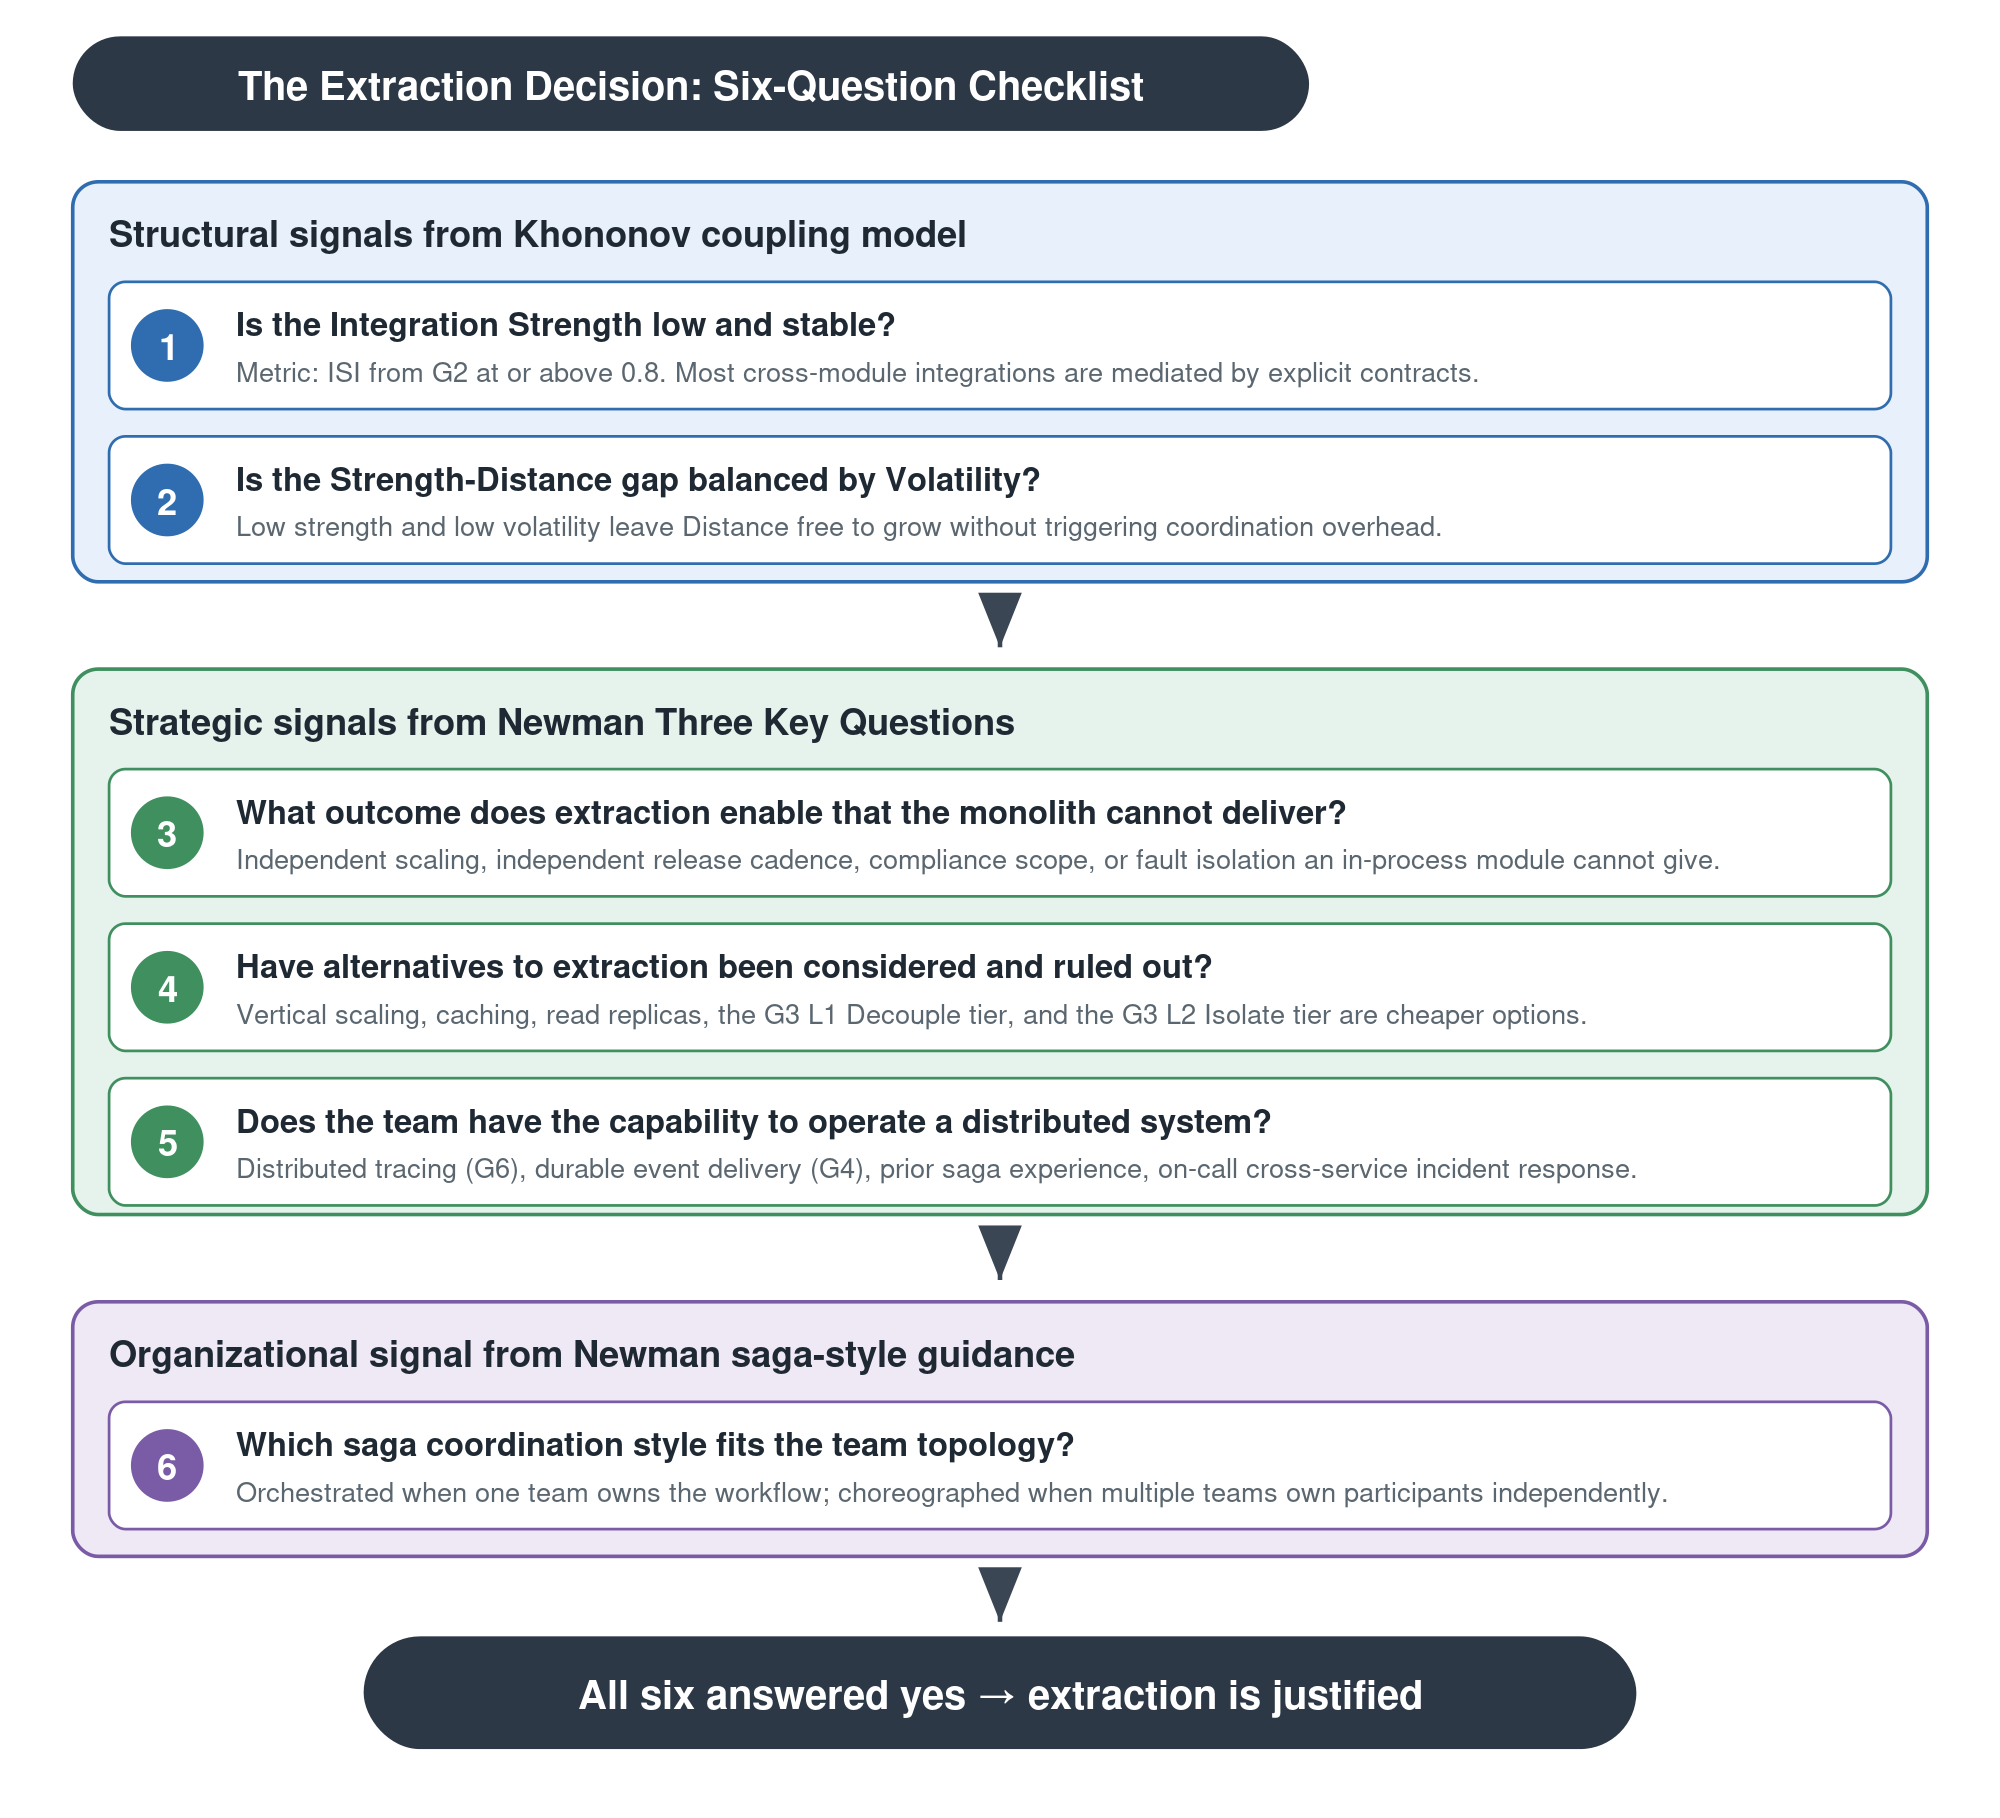
\includegraphics[width=\linewidth]{Cap4/guidelines/extraction_decision_flowchart.png}
  \caption{The Extraction Decision as a six-question checklist}
  \label{fig:extraction-decision-flowchart}
\end{figure}

\subsection*{Why a Distinct Decision Framework}

The six guidelines G1 to G6 describe \emph{how} to build a modular monolith that remains extractable. The Extraction Decision answers \emph{when} the cost of extraction is justified. The two questions are coupled but not equivalent. A team can satisfy G1 to G6 in full and still be wrong to extract, if the outcome can be delivered by the monolith without the operational overhead of a distributed system. Conversely, a team can be right to extract and still fail, if G4's Anti-Corruption Layers, saga orchestration, and event-streaming infrastructure are not in place to absorb the change. The decision framework separates the two questions so that each is treated on its own merits.

This separation also addresses a recurring finding from the verification phase. Several participants observed that the guidelines, taken individually, can be read as a prescription to extract: each one strengthens the readiness signal, and readiness can be mistaken for a recommendation. The Extraction Decision makes the recommendation question explicit and binds it to outcomes that the monolith cannot deliver. Readiness becomes a precondition for extraction, not a trigger.

\subsection*{Worked Application: The Tiny Store Payments Module}

The Tiny Store reference implementation~\cite{tinystore2026} is used throughout this chapter as a concrete carrier for the guidelines. The Extraction Decision can be applied to its payments module as a worked example. The application below walks through the six questions in order.

\paragraph*{Questions one and two (structural).} The payments module is integrated with orders, inventory, and shipments through Kafka topics, which are contract-level integration points in Khononov's taxonomy. Static analysis of the cross-module references in the repository returns $\text{ISI} = 0.92$, well above the target of $0.8$, which satisfies question one. Distance between payments and the rest of the monolith is high: payments carries dedicated regulatory constraints (PCI scope) that the other modules do not, which makes organizational separation natural. Volatility is low: the payment-confirmed event contract has not changed in six months. Low strength and low volatility leave room for distance to grow without triggering coordination overhead, which satisfies Khononov's balance condition and answers question two.

\paragraph*{Question three (outcome).} Extracting payments allows the PCI compliance audit to scope a single deployed service rather than the full monolith, which reduces compliance overhead in a way that no intra-monolith mechanism can replicate. The outcome is concrete and the monolith cannot deliver it.

\paragraph*{Question four (alternatives).} The cheaper alternatives are ruled out by the same compliance requirement. The L2 Isolate tier of G3 (a dedicated database schema while keeping a single deployment target) would isolate persistence but not deployment, and PCI requires separate deployment targets. Vertical scaling and caching do not affect compliance scope.

\paragraph*{Question five (capability).} The team is prepared for distributed operation. Distributed tracing is in place through OpenTelemetry, the team has prior experience with Temporal sagas, and the on-call rotation already monitors the Kafka topics that the extracted service will continue to publish to.

\paragraph*{Question six (saga style).} The choreographed style is selected. Orders and shipments are owned by different teams that should not be forced to coordinate releases with payments after the extraction; an orchestrated saga would impose that coordination through the orchestrator's interface.

\paragraph*{Verdict.} All six questions are answered in the affirmative. The payments module is a justified extraction candidate.

\paragraph*{Counter-example: the inventory module.} The same analysis applied to the inventory module returns a different verdict. Inventory passes the structural questions (ISI is high, contracts are stable), but it fails question three. The required scaling is already delivered by the G3 L1 Decouple tier (asynchronous boundaries within the monolith), and extraction would add the operational cost of distribution without delivering an outcome the monolith cannot match. Inventory remains in the monolith.

Figure~\ref{fig:extraction-decision-worked} consolidates the two analyses side by side. Payments passes every question and is extracted; inventory fails question three and stops the evaluation there, because the remaining questions cannot change the verdict.

\begin{figure}[H]
  \centering
  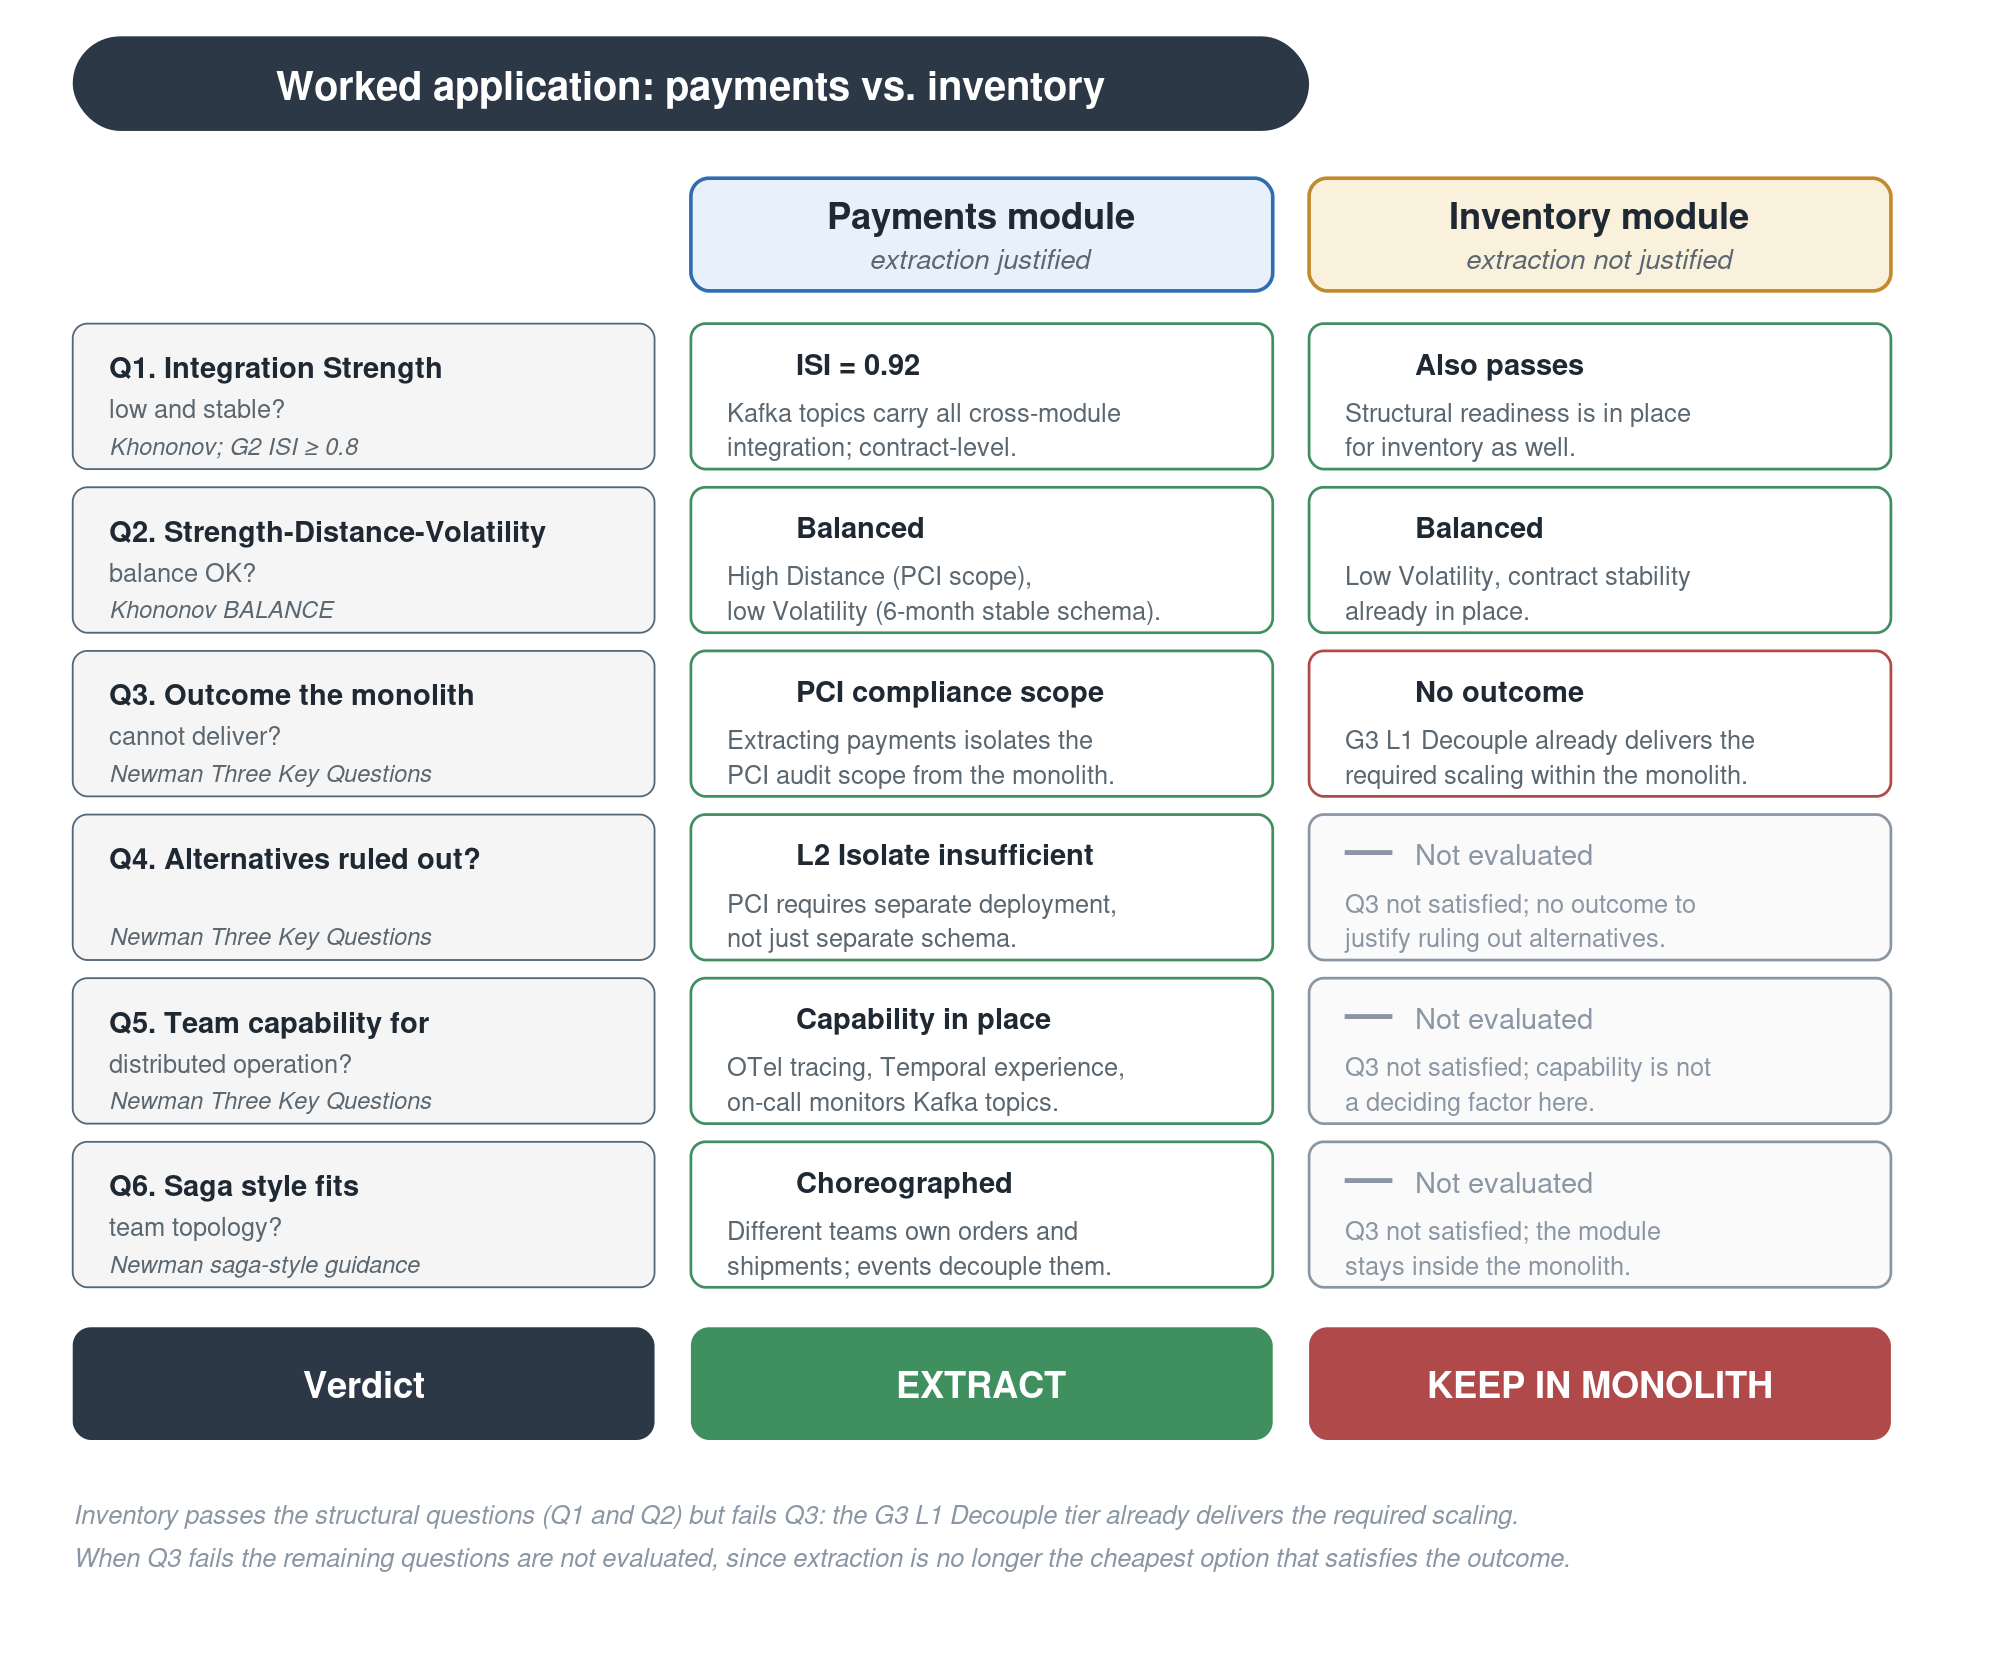
\includegraphics[width=\linewidth]{Cap4/guidelines/extraction_decision_worked_application.png}
  \caption{The Extraction Decision applied to the Tiny Store payments and inventory modules}
  \label{fig:extraction-decision-worked}
\end{figure}

\subsection*{Position in the Guideline Set}

The Extraction Decision is not a seventh guideline; it is a synthesis layer that activates the existing six. G1 and G2 supply the structural visibility and the Integration Strength signal of question one. G3 supplies the readiness gate $\varepsilon_m$ and the intermediate tiers (L1 Decouple, L2 Isolate) that question four uses as the formal alternatives to extraction. G4 supplies the operational guarantees (Anti-Corruption Layers, the saga catalog from Foundations for the Operational Fit Dimension applied through G4, durable event delivery) that questions five and six rely on. G6 supplies the cross-module observability without which the team-capability claim of question five collapses. G5 does not enter the decision itself; its role is downstream, because the deployment pipeline must already support a multi-target topology at the moment of execution for the extracted service to reach production.

The framework is, in this sense, the use case the guidelines were designed to serve.
